\documentclass[12pt,a4paper]{article}

% ─── Pacotes ─────────────────────────────────────────────────────────────────
\usepackage[utf8]{inputenc}
\usepackage[T1]{fontenc}
\usepackage[portuguese]{babel}
\usepackage{geometry}
\usepackage{graphicx}
\usepackage{hyperref}
\usepackage{booktabs}
\usepackage{longtable}
\usepackage{enumitem}
\usepackage{listings}
\usepackage{xcolor}
\usepackage{titlesec}
\usepackage{fancyhdr}
\usepackage{setspace}
\usepackage{microtype}
\usepackage{parskip}
\usepackage{caption}
\usepackage{float}
\usepackage{amsmath}
\usepackage{array}
\usepackage{multirow}

% ─── Geometria ───────────────────────────────────────────────────────────────
\geometry{
  top=3cm, bottom=2cm,
  left=3cm, right=2cm
}

% ─── Cores ───────────────────────────────────────────────────────────────────
\definecolor{codebg}{RGB}{245,245,245}
\definecolor{codecomment}{RGB}{106,153,85}
\definecolor{codestring}{RGB}{206,145,120}
\definecolor{codekeyword}{RGB}{86,156,214}
\definecolor{primary}{RGB}{30,80,160}
\definecolor{accent}{RGB}{200,60,30}

% ─── Hyperref ────────────────────────────────────────────────────────────────
\hypersetup{
  colorlinks=true,
  linkcolor=primary,
  urlcolor=primary,
  citecolor=primary,
  pdftitle={Relatório de Arquitetura — BarberManager},
  pdfauthor={Miguel Huertas}
}

% ─── Listings (código Pascal) ─────────────────────────────────────────────────
\lstdefinelanguage{Pascal}{
  keywords={begin,end,var,function,procedure,type,record,class,
            interface,implementation,uses,unit,program,if,then,else,
            while,do,for,to,repeat,until,case,of,try,except,finally,
            raise,with,inherited,override,virtual,property,published,
            private,protected,public,constructor,destructor,nil,not,
            and,or,xor,div,mod,in,is,as,string,integer,boolean,
            TFDConnection,TFDQuery,THorse,THorseRequest,THorseResponse,
            TProc,THashSHA2},
  sensitive=false,
  morecomment=[l]{//},
  morecomment=[s]{\{}{\}},
  morestring=[b]',
  morestring=[b]"
}

\lstset{
  language=Pascal,
  backgroundcolor=\color{codebg},
  basicstyle=\ttfamily\small,
  keywordstyle=\color{codekeyword}\bfseries,
  commentstyle=\color{codecomment}\itshape,
  stringstyle=\color{codestring},
  breaklines=true,
  breakatwhitespace=true,
  frame=single,
  rulecolor=\color{gray!40},
  numbers=left,
  numberstyle=\tiny\color{gray},
  tabsize=2,
  captionpos=b,
  showstringspaces=false
}

% ─── Cabeçalho / Rodapé ──────────────────────────────────────────────────────
\pagestyle{fancy}
\fancyhf{}
\fancyhead[L]{\small\textit{BarberManager — Relatório de Arquitetura}}
\fancyhead[R]{\small\textit{2025}}
\fancyfoot[C]{\thepage}
\renewcommand{\headrulewidth}{0.4pt}

% ─── Títulos ─────────────────────────────────────────────────────────────────
\titleformat{\section}
  {\large\bfseries\color{primary}}{\thesection}{1em}{}[\titlerule]
\titleformat{\subsection}
  {\normalsize\bfseries\color{primary!80}}{\thesubsection}{1em}{}
\titleformat{\subsubsection}
  {\normalsize\bfseries}{\thesubsubsection}{1em}{}

\setcounter{secnumdepth}{3}
\setcounter{tocdepth}{3}

% ═════════════════════════════════════════════════════════════════════════════
\begin{document}

% ─── Capa ────────────────────────────────────────────────────────────────────
\begin{titlepage}
  \centering
  \vspace*{2cm}

  {\Large\bfseries Universidade — Disciplina de Programação Web\par}
  \vspace{0.5cm}
  {\large Curso de Tecnologia em Análise e Desenvolvimento de Sistemas\par}

  \vfill

  {\Huge\bfseries\color{primary} BarberManager\par}
  \vspace{0.4cm}
  {\LARGE Relatório de Arquitetura de Software\par}

  \vspace{1.5cm}
  \rule{0.8\textwidth}{0.4pt}
  \vspace{1.5cm}

  \begin{tabular}{ll}
    \textbf{Autor:}       & Miguel Huertas \\[4pt]
    \textbf{Disciplina:}  & Programação Web \\[4pt]
    \textbf{Semestre:}    & 5.º Semestre \\[4pt]
    \textbf{Data:}        & Junho de 2025 \\
  \end{tabular}

  \vfill

  {\small\textit{Documento gerado a partir do código-fonte do projecto BarberManager}\par}
\end{titlepage}

% ─── Resumo ──────────────────────────────────────────────────────────────────
\newpage
\section*{Resumo}
\addcontentsline{toc}{section}{Resumo}

Este relatório documenta a arquitetura de software do sistema \textbf{BarberManager}, um sistema de gestão de barbearia desenvolvido como projecto académico da disciplina de Programação Web. O sistema compreende duas camadas independentes que partilham a mesma base de dados Firebird~3.0: uma aplicação nativa Desktop/Mobile construída com Delphi~12 e FireMonkey (FMX), e um Web App composto por uma REST API em Horse (Object Pascal) com frontend em HTML/CSS/JS puro.

O documento analisa a arquitectura segundo o modelo C4, avalia a conformidade com os princípios SOLID, Clean Code e DRY, identifica métricas de qualidade observadas no código e apresenta um roadmap evolutivo para o sistema.

\textbf{Palavras-chave:} Delphi, FireMonkey, Horse, Firebird, REST API, SOLID, Clean Code, C4 Model, Arquitetura em Camadas.

% ─── Sumário ─────────────────────────────────────────────────────────────────
\newpage
\tableofcontents

% ─────────────────────────────────────────────────────────────────────────────
\newpage
\section{Visão Geral do Sistema}

\subsection{Descrição do Projecto}

O \textbf{BarberManager} é um sistema completo e moderno para a gestão de barbearias. O projecto aplica Engenharia de Software, UI/UX Design moderno e Arquitectura em Camadas para oferecer:

\begin{itemize}
  \item \textbf{Painel do Cliente} — agendamento online, catálogo de serviços, avaliações e perfil editável.
  \item \textbf{Dashboard do Administrador} — KPIs em tempo real, gestão de agenda, serviços, clientes, relatório financeiro e configurações da barbearia.
\end{itemize}

O sistema cobre o ciclo completo de vida de um agendamento: criação pelo cliente, acompanhamento do status (PENDENTE → EM\_ANDAMENTO → CONCLUÍDO), avaliação pós-serviço e reflecção nas métricas de faturamento.

\subsection{Stack Tecnológica}

\begin{table}[H]
\centering
\caption{Stack tecnológica do BarberManager}
\begin{tabular}{@{}lp{9cm}@{}}
\toprule
\textbf{Componente} & \textbf{Detalhe} \\
\midrule
IDE & Delphi 12 Athens \\
App Nativo & FireMonkey (FMX) — Windows, Android, iOS \\
REST API & Horse framework — servidor HTTP porta 9000 \\
Frontend Web & HTML/CSS/JS puro — SPA \textit{single-file} (\texttt{index.html}) \\
Base de Dados & Firebird 3.0 (protocolo Local, \texttt{fbclient.dll}) \\
Acesso a Dados & FireDAC — conexão \textit{per-request} na API; \textit{singleton} no app nativo \\
Segurança & SHA-256 uppercase (\texttt{THashSHA2}) para passwords \\
Deploy & ngrok Tunnel — domínio fixo \texttt{humid-boots-posted.ngrok-free.dev} \\
Linguagem & Object Pascal \\
\bottomrule
\end{tabular}
\end{table}

\subsection{Objectivos Arquitectónicos}

Os objectivos que guiaram as decisões de design foram:

\begin{enumerate}
  \item \textbf{Separação de responsabilidades} — camada de dados, lógica de negócio e apresentação distintas.
  \item \textbf{Thread-safety} — Horse é multi-thread; cada request obtém a sua própria conexão à BD.
  \item \textbf{Resiliência} — padrões defensivos no FireDAC (LEFT JOIN + COALESCE, CAST de campos TIME) para evitar Access Violations em dados nulos.
  \item \textbf{Zero dependências externas no frontend} — HTML/CSS/JS puro, sem frameworks JS.
  \item \textbf{Deploy simples} — um único executável serve a API e o frontend estático.
\end{enumerate}

% ─────────────────────────────────────────────────────────────────────────────
\newpage
\section{Arquitectura C4}

O modelo C4 (\textit{Context, Containers, Components, Code}) foi adoptado para documentar a arquitectura em quatro níveis de abstracção crescente.

\subsection{Nível 1 — Diagrama de Contexto}

O sistema interage com dois tipos de actores externos:

\begin{itemize}
  \item \textbf{Cliente da Barbearia} — acede ao Web App via browser ou à app nativa via dispositivo móvel/desktop para consultar serviços, agendar, avaliar e gerir o seu perfil.
  \item \textbf{Barbeiro / Administrador} — acede ao Dashboard Admin via browser ou app nativa para gerir agenda, serviços, clientes e relatórios financeiros.
\end{itemize}

O sistema comunica exclusivamente com a base de dados Firebird~3.0 local. O túnel ngrok actua como proxy reverso para expor a API publicamente sem abertura de portas na rede.

\begin{figure}[H]
  \centering
  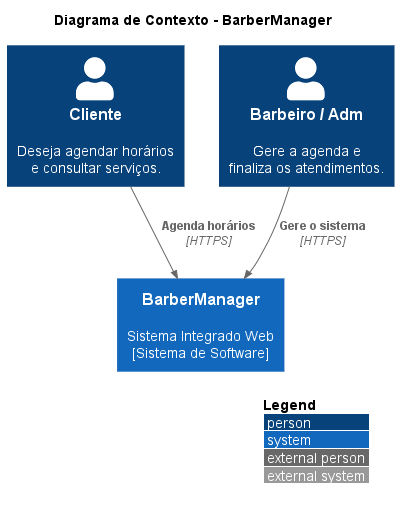
\includegraphics[width=0.85\textwidth]{../Diagramas_C4/diagrama_contexto.png}
  \caption{Diagrama de Contexto C4 — BarberManager}
\end{figure}

\subsection{Nível 2 — Diagrama de Containers}

O sistema é composto por dois containers principais e um container de dados:

\begin{table}[H]
\centering
\caption{Containers do BarberManager}
\begin{tabular}{@{}llp{6.5cm}@{}}
\toprule
\textbf{Container} & \textbf{Tecnologia} & \textbf{Responsabilidade} \\
\midrule
App Nativo FMX & Delphi 12 / FMX & Interface nativa Desktop/Mobile para cliente e admin \\
Horse REST API & Object Pascal / Horse & Servidor HTTP porta 9000; serve REST API + frontend HTML \\
Firebird 3.0 & Firebird / FireDAC & Base de dados relacional local \\
ngrok Tunnel & ngrok & Proxy reverso — expõe porta 9000 publicamente \\
\bottomrule
\end{tabular}
\end{table}

\begin{figure}[H]
  \centering
  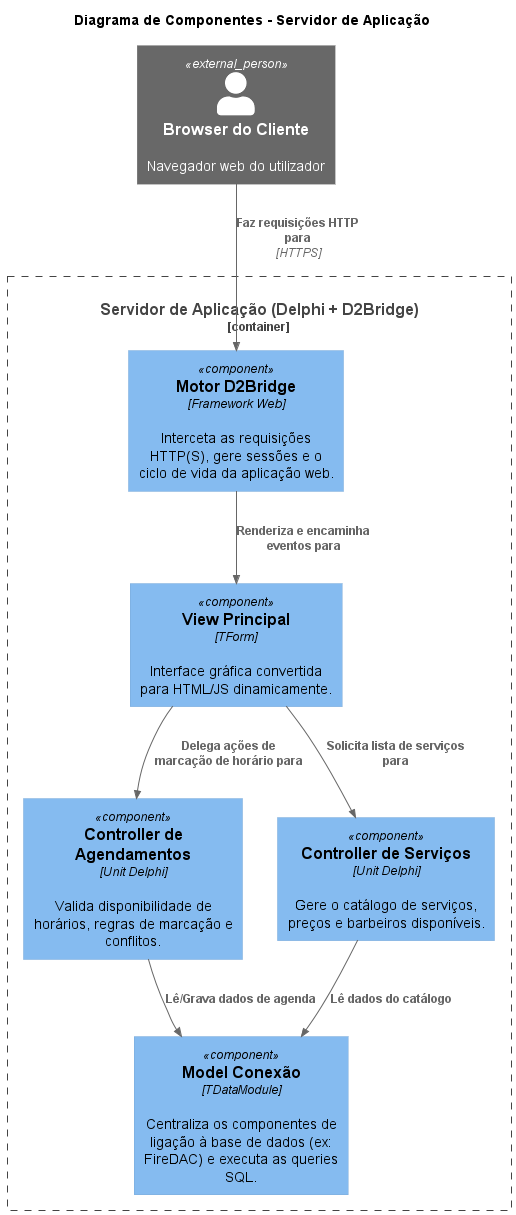
\includegraphics[width=0.85\textwidth]{../Diagramas_C4/diagrama_componentes.png}
  \caption{Diagrama de Componentes C4 — BarberManager}
\end{figure}

\subsection{Nível 3 — Diagrama de Componentes (Horse REST API)}

A REST API está organizada em \textit{units} Pascal com responsabilidades bem delimitadas:

\begin{table}[H]
\centering
\caption{Componentes da REST API}
\begin{tabular}{@{}lp{9cm}@{}}
\toprule
\textbf{Unit} & \textbf{Responsabilidade} \\
\midrule
\texttt{API.Conexao} & Factory \texttt{CreateConnection} — nova \texttt{TFDConnection} por request \\
\texttt{API.Auth} & \texttt{POST /api/auth/login}, \texttt{POST /api/auth/cadastro} \\
\texttt{API.Agendamentos} & CRUD agendamentos + \texttt{AutoAtualizarStatus} \\
\texttt{API.Avaliacoes} & GET/POST avaliações; actualização de \texttt{AVALIACAO\_MEDIA} \\
\texttt{API.Barbeiros} & \texttt{GET /api/barbeiros} \\
\texttt{API.Clientes} & Listagem e toggle ativo/inativo \\
\texttt{API.Dashboard} & KPIs, timeline, relatório financeiro \\
\texttt{API.Servicos} & CRUD completo de serviços \\
\texttt{API.Usuarios} & Perfil editável: GET + PUT \\
\bottomrule
\end{tabular}
\end{table}

\subsection{Nível 4 — Padrões de Código}

\subsubsection{Padrão per-request (thread-safety)}

O Horse processa cada HTTP request numa thread separada. Para garantir thread-safety, \textbf{nunca} é partilhada uma conexão global:

\begin{lstlisting}[caption={Padrão per-request em API.Conexao.pas}]
function CreateConnection: TFDConnection;
var
  Conn: TFDConnection;
begin
  Conn := TFDConnection.Create(nil);
  Conn.Params.DriverID := 'FB';
  Conn.Params.Database := DB_PATH;
  Conn.Params.UserName := 'SYSDBA';
  Conn.Params.Password := 'masterkey';
  Conn.TxOptions.Isolation := xiReadCommitted;
  Conn.Connected := True;
  Result := Conn;
end;

// Uso em cada handler:
Conn := CreateConnection;
try
  // ... queries ...
finally
  Conn.Free;
end;
\end{lstlisting}

\subsubsection{Padrão defensivo de query}

Para evitar Access Violations no FireDAC com resultados vazios ou FKs órfãs:

\begin{lstlisting}[caption={Padrão RDB\$DATABASE LEFT JOIN para agregados}]
SELECT
  COALESCE(Q.TOTAL, 0)       AS TOTAL,
  COALESCE(Q.FATURAMENTO, 0) AS FATURAMENTO
FROM RDB$DATABASE
LEFT JOIN (
  SELECT COUNT(*) AS TOTAL, SUM(VALOR_COBRADO) AS FATURAMENTO
  FROM TB_AGENDAMENTOS
  WHERE CAST(DT_AGENDAMENTO AS DATE) = CAST(CURRENT_DATE AS DATE)
    AND STATUS = 'CONCLUIDO'
) Q ON 1=1
\end{lstlisting}

Este padrão garante sempre exactamente uma linha no resultado, impedindo que o FireDAC perca os aliases de campos em resultados vazios.

% ─────────────────────────────────────────────────────────────────────────────
\newpage
\section{Modelo de Dados}

\subsection{Diagrama Entidade-Relacionamento}

O esquema da base de dados Firebird~3.0 compreende sete tabelas principais:

\begin{table}[H]
\centering
\caption{Tabelas da base de dados}
\begin{tabular}{@{}lp{10cm}@{}}
\toprule
\textbf{Tabela} & \textbf{Colunas principais} \\
\midrule
\texttt{TB\_USUARIOS} & ID, NOME\_COMPLETO, EMAIL, SENHA\_HASH (SHA-256 uppercase), PERFIL ('ADMIN'/'CLIENTE'), ATIVO, DT\_CADASTRO, TELEFONE \\
\texttt{TB\_SERVICOS} & ID, NOME, DESCRICAO, PRECO, DURACAO\_MIN, CATEGORIA\_ID (FK), BADGE, ATIVO \\
\texttt{TB\_CATEGORIAS} & ID, NOME ('Cabelo', 'Barba', 'Estética') \\
\texttt{TB\_BARBEIROS} & ID, USUARIO\_ID (FK), CARGO, AVALIACAO\_MEDIA, ATIVO \\
\texttt{TB\_AGENDAMENTOS} & ID, CLIENTE\_ID, BARBEIRO\_ID, SERVICO\_ID, DT\_AGENDAMENTO, HR\_INICIO (TIME), HR\_FIM (TIME), STATUS, VALOR\_COBRADO \\
\texttt{TB\_AVALIACOES} & ID, AGENDAMENTO\_ID (FK), CLIENTE\_ID (FK), BARBEIRO\_ID (FK), NOTA (1--5), COMENTARIO, DT\_AVALIACAO \\
\texttt{TB\_CONFIGURACOES} & ID, CHAVE (UNIQUE), VALOR, DESCRICAO \\
\bottomrule
\end{tabular}
\end{table}

\subsection{Ciclo de Vida do Agendamento}

O campo \texttt{STATUS} em \texttt{TB\_AGENDAMENTOS} segue a máquina de estados:

\[
\texttt{PENDENTE} \;\longrightarrow\; \texttt{EM\_ANDAMENTO} \;\longrightarrow\; \texttt{CONCLUIDO}
\]
\[
\texttt{PENDENTE} \;\longrightarrow\; \texttt{CANCELADO}
\]

A transição automática é executada pelo middleware \texttt{AutoAtualizarStatus} a cada GET request, com três UPDATEs sequenciais:

\begin{enumerate}
  \item PENDENTE → EM\_ANDAMENTO quando \texttt{HR\_INICIO} $\leq$ \texttt{CURRENT\_TIME} (hoje).
  \item EM\_ANDAMENTO → CONCLUIDO quando \texttt{HR\_FIM} passou ou é dia anterior.
  \item PENDENTE/EM\_ANDAMENTO → CONCLUIDO para dias anteriores (\textit{missed appointments}).
\end{enumerate}

% ─────────────────────────────────────────────────────────────────────────────
\newpage
\section{Princípios SOLID — Análise}

\subsection{S — Single Responsibility Principle (SRP)}

\textbf{Conformidade: Alta.}

Cada \textit{unit} da API tem uma única responsabilidade bem definida. \texttt{API.Auth} lida exclusivamente com autenticação; \texttt{API.Dashboard} serve apenas os endpoints de métricas; \texttt{API.Conexao} fornece exclusivamente a factory de conexões.

No lado FMX, os \textit{frames} (Serviços, Agenda, Clientes, Financeiro, Configurações) encapsulam cada secção do dashboard de forma independente, respeitando o SRP.

\textbf{Violação parcial observada:} \texttt{View.Principal.pas} concentra login, cadastro, home do cliente e ecrã de agendamento num único formulário. Esta opção foi deliberada para compatibilidade com a navegação por tabs do FMX, mas aumenta o acoplamento interno deste ficheiro.

\subsection{O — Open/Closed Principle (OCP)}

\textbf{Conformidade: Média.}

A adição de novos endpoints no Horse é feita criando uma nova \textit{unit} \texttt{API.X.pas} e registando as rotas em \texttt{BarberManagerAPI.dpr}, sem modificar as units existentes — comportamento aberto para extensão, fechado para modificação.

\textbf{Oportunidade de melhoria:} A lógica de filtros em \texttt{API.Agendamentos.RotaListar} constrói a cláusula \texttt{WHERE} por concatenação condicional de strings. A adição de novos filtros obriga a modificar o método existente, violando o OCP.

\subsection{L — Liskov Substitution Principle (LSP)}

\textbf{N/A — baixo uso de herança.}

O projecto usa essencialmente composição. Os \textit{frames} FMX herdam de \texttt{TFrame} mas não redefinem comportamento herdado de forma incompatível. O LSP não é uma preocupação activa neste contexto.

\subsection{I — Interface Segregation Principle (ISP)}

\textbf{Conformidade: Alta.}

Cada \textit{unit} exporta apenas as funções necessárias para o seu contrato. \texttt{API.Agendamentos} exporta \texttt{RegistrarRotas} e \texttt{AutoAtualizarStatus} — nada mais. O consumidor (\texttt{BarberManagerAPI.dpr}) não é forçado a depender de métodos que não usa.

\subsection{D — Dependency Inversion Principle (DIP)}

\textbf{Conformidade: Baixa — típica de Pascal procedural.}

As dependências entre units são estáticas (cláusula \texttt{uses}). Não existe injecção de dependências nem interfaces abstractas entre camadas. \texttt{API.Agendamentos} depende directamente de \texttt{API.Conexao}, e os handlers dependem directamente do FireDAC.

Num contexto académico com linguagem procedural como Object Pascal, esta limitação é esperada e aceitável. A mitigação adoptada é manter cada \textit{unit} coesa e com baixo acoplamento externo.

% ─────────────────────────────────────────────────────────────────────────────
\newpage
\section{Clean Code — Análise}

\subsection{Nomenclatura}

O projecto adopta convenções consistentes:

\begin{itemize}
  \item Prefixo \texttt{T} para tipos (\texttt{TdmConexao}, \texttt{TFDQuery}).
  \item Prefixo \texttt{F} para campos privados de formulário (\texttt{FUsuarioID}, \texttt{FUsuarioNome}).
  \item Prefixo \texttt{Rota} para handlers de endpoint (\texttt{RotaListar}, \texttt{RotaCriar}).
  \item Nomes de tabelas em maiúsculas com prefixo \texttt{TB\_} (\texttt{TB\_AGENDAMENTOS}).
  \item Parâmetros de query em maiúsculas (\texttt{:STATUS}, \texttt{:CLIENTE\_ID}).
\end{itemize}

\textbf{Ponto positivo:} nomes como \texttt{AutoAtualizarStatus}, \texttt{CreateConnection} e \texttt{RegistrarRotas} comunicam intenção sem necessidade de comentário.

\subsection{Funções Pequenas e Focadas}

Cada handler de rota (\texttt{Rota*}) executa uma única operação HTTP. Os métodos de auto-atualização de status são separados do handler principal, permitindo reutilização como middleware.

\subsection{Tratamento de Erros}

O padrão \texttt{try/except/finally} é aplicado consistentemente:

\begin{lstlisting}[caption={Padrão de tratamento de erros com transação}]
Conn.StartTransaction;
try
  QInsert.ExecSQL;
  QUpdate.ExecSQL;
  Conn.Commit;
except
  Conn.Rollback;
  raise;
end;
\end{lstlisting}

O middleware \texttt{AutoAtualizarStatus} usa \textit{silent except} — qualquer falha na atualização automática de status é silenciada para não interromper o request principal do cliente.

\subsection{Evitar Comentários Desnecessários}

O código não contém comentários óbvios ou que descrevam o \textit{o quê}. Os comentários existentes documentam apenas decisões não óbvias (ex.: razão do padrão \texttt{RDB\$DATABASE LEFT JOIN}, necessidade de \texttt{CAST} no campo \texttt{TIME}).

\subsection{Pontos de Melhoria (Clean Code)}

\begin{itemize}
  \item \texttt{View.Principal.pas} tem métodos longos (ex.: \texttt{CarregarServicos}, \texttt{CriarSlots}) que poderiam ser decompostos.
  \item A construção de JSON por concatenação de strings em alguns handlers poderia ser substituída por \texttt{TJSONObject} para maior legibilidade.
  \item Alguns magic numbers (ex.: \texttt{Tag = 99}, \texttt{Tag = 88}) estão documentados no \texttt{CLAUDE.md} mas não em constantes nomeadas no código.
\end{itemize}

% ─────────────────────────────────────────────────────────────────────────────
\newpage
\section{Princípio DRY — Don't Repeat Yourself}

\subsection{Boas Práticas Observadas}

\subsubsection{Factory de Conexão}

A função \texttt{CreateConnection} em \texttt{API.Conexao.pas} elimina duplicação: toda a configuração da conexão (DriverID, Database, UserName, Password, CharacterSet, TxOptions) está num único local. Os 9 handlers da API invocam \texttt{CreateConnection} sem conhecer os detalhes.

\subsubsection{Auto-atualização de Status como Middleware}

\texttt{AutoAtualizarStatus} é invocado uma única vez no middleware Horse (antes de todas as rotas GET), em vez de ser duplicado em cada endpoint que necessite de dados actualizados.

\subsubsection{Padrão de Query Reutilizável}

O padrão \texttt{RDB\$DATABASE LEFT JOIN} é aplicado de forma consistente em todos os endpoints de agregados (\texttt{/api/dashboard/kpis}, \texttt{/api/dashboard/financeiro}), evitando que cada developer reinvente a solução para o problema do FireDAC com resultados vazios.

\subsection{Violações DRY Identificadas}

\begin{itemize}
  \item \textbf{Lógica de hash SHA-256} — a expressão \texttt{UpperCase(THashSHA2.GetHashString(senha, SHA256))} está duplicada em \texttt{API.Auth} (login e cadastro) e em \texttt{API.Usuarios} (alteração de senha). Uma função utilitária \texttt{HashSenha(s: string): string} eliminaria a duplicação.

  \item \textbf{Blocos de header CORS} — os headers \texttt{Access-Control-Allow-Origin}, \texttt{Access-Control-Allow-Methods} e \texttt{Access-Control-Allow-Headers} estão definidos no middleware central, mas a sua gestão está misturada com o shortcircuit do OPTIONS no mesmo bloco. A separação em funções distintas melhoraria a clareza.

  \item \textbf{Validação de campos obrigatórios} — a verificação de campos vazios (\texttt{if Trim(campo) = ''}) está dispersa em múltiplos handlers sem abstracção. Uma função \texttt{ValidarCamposObrigatorios} centralizaria esta lógica.
\end{itemize}

% ─────────────────────────────────────────────────────────────────────────────
\newpage
\section{Boas Práticas de Arquitetura}

\subsection{Separação Frontend/Backend}

O frontend em HTML/CSS/JS puro consome a API exclusivamente via \texttt{fetch()} com \texttt{API\_BASE = ''} (URLs relativas). Como o \texttt{.exe} serve tanto a API quanto o \texttt{index.html} no mesmo processo e porta, não existe problema de CORS em produção. O middleware CORS está presente apenas para suportar desenvolvimento local com Live Server.

\subsection{Stateless API}

A API Horse é completamente \textit{stateless}: não existe sessão no servidor. A autenticação é feita por login, o servidor retorna \texttt{\{id, nome, email, perfil\}}, e o cliente persiste estes dados em \texttt{localStorage}. Cada request subsequente inclui o \texttt{userId} no path ou query string conforme necessário.

\subsection{Gestão de Estado no Frontend}

O SPA usa um objeto \texttt{currentUser} em memória (populado do \texttt{localStorage} no carregamento) e actualiza a UI via funções de renderização. O badge de notificações usa \texttt{localStorage.lastSeenNotifId} para persistir o estado entre sessões sem necessidade de tabela de sessões no servidor.

\subsection{Deploy sem Servidor Dedicado}

O sistema corre num único PC Windows sem IP fixo, exposto publicamente via \textbf{ngrok} com domínio permanente \texttt{humid-boots-posted.ngrok-free.dev}. O script \texttt{start-barbermanager.ps1} automatiza o arranque dos dois processos em janelas PowerShell separadas.

\subsection{Segurança}

\begin{itemize}
  \item Passwords armazenadas como \textbf{SHA-256 uppercase} — nunca em texto claro.
  \item Validação de whitelist para o campo \texttt{STATUS} (\texttt{PENDENTE/EM\_ANDAMENTO/CONCLUIDO/CANCELADO}) antes de qualquer UPDATE.
  \item Verificação de unicidade de email (excluindo o próprio utilizador) antes de actualizar o perfil.
  \item Verificação de duplicado de avaliação antes de INSERT para evitar dupla avaliação do mesmo agendamento.
\end{itemize}

\textbf{Oportunidades de melhoria:}
\begin{itemize}
  \item Implementar autenticação por JWT para eliminar a dependência de \texttt{userId} no query string.
  \item Adicionar rate limiting no Horse para proteger os endpoints de autenticação.
  \item Migrar para HTTPS nativo (actualmente o TLS é fornecido pelo ngrok).
\end{itemize}

% ─────────────────────────────────────────────────────────────────────────────
\newpage
\section{Métricas de Qualidade}

\subsection{Métricas Estruturais}

\begin{table}[H]
\centering
\caption{Métricas do projecto BarberManager}
\begin{tabular}{@{}lrr@{}}
\toprule
\textbf{Métrica} & \textbf{Valor} & \textbf{Referência} \\
\midrule
Units Pascal (API) & 9 & — \\
Units Pascal (FMX) & 8+ & — \\
Endpoints REST & 20 & — \\
Tabelas BD & 7 & — \\
Linhas de código (estimativa) & $\sim$5\,000 & — \\
Cobertura de testes automatizados & 0\% & (ver roadmap) \\
Acoplamento entre units API & Baixo & $\leq$2 dependências/unit \\
Coesão por unit & Alta & 1 responsabilidade/unit \\
\bottomrule
\end{tabular}
\end{table}

\subsection{Métricas de Robustez}

\begin{table}[H]
\centering
\caption{Padrões defensivos implementados}
\begin{tabular}{@{}lll@{}}
\toprule
\textbf{Padrão} & \textbf{Aplicado em} & \textbf{Problema evitado} \\
\midrule
LEFT JOIN + COALESCE & Todos os JOINs da API & AV no FireDAC com FK órfã \\
CAST(HR AS VARCHAR(13)) & Campos TIME & AV no FireDAC com campo TIME \\
RDB\$DATABASE LEFT JOIN & Agregados com possível zero linhas & Campo não encontrado no FireDAC \\
Silent except & AutoAtualizarStatus & Falha silenciosa no middleware \\
try/finally Conn.Free & Todos os handlers & Fuga de memória/conexão \\
\bottomrule
\end{tabular}
\end{table}

\subsection{Complexidade Ciclomática}

Os handlers da API têm complexidade ciclomática baixa a média (estimada entre 3 e 8), com excepção de:

\begin{itemize}
  \item \texttt{API.Agendamentos.RotaListar} — construção condicional do \texttt{WHERE} com 4 filtros opcionais (CC $\approx$ 8).
  \item \texttt{View.Principal.pas} — métodos de renderização de cards e calendário (CC $\approx$ 10--15).
\end{itemize}

Estes valores estão dentro de limites aceitáveis para código académico, mas seria recomendável decomposição para manutenção a longo prazo.

% ─────────────────────────────────────────────────────────────────────────────
\newpage
\section{Roadmap Evolutivo}

\subsection{Estado Actual (Junho 2025)}

Todas as funcionalidades planeadas para o projecto académico estão implementadas e funcionais:

\begin{table}[H]
\centering
\caption{Estado do projecto}
\begin{tabular}{@{}lc@{}}
\toprule
\textbf{Módulo} & \textbf{Estado} \\
\midrule
App FMX — Login, Cadastro, Home, Agendamento & \checkmark \\
App FMX — Carrinho + Avaliação & \checkmark \\
App FMX — Dashboard Admin completo & \checkmark \\
REST API — todos os endpoints (porta 9000) & \checkmark \\
Web SPA — Área Cliente completa & \checkmark \\
Web SPA — Área Admin completa & \checkmark \\
Auto-status middleware & \checkmark \\
Deploy via ngrok (domínio fixo) & \checkmark \\
\bottomrule
\end{tabular}
\end{table}

\subsection{Fase 10 — Testes Automatizados}

\begin{itemize}
  \item Implementar testes de integração para os endpoints da REST API usando \texttt{DUnitX} ou scripts \texttt{curl} automatizados.
  \item Cobrir os casos de erro: email duplicado, status inválido, avaliação duplicada.
  \item Meta: cobertura de 60\% nos endpoints críticos (auth, agendamentos, avaliações).
\end{itemize}

\subsection{Fase 11 — Autenticação JWT}

\begin{itemize}
  \item Substituir o \texttt{userId} em query string por JWT Bearer token no header \texttt{Authorization}.
  \item Implementar middleware de validação de token no Horse.
  \item Adicionar refresh token com TTL configurável em \texttt{TB\_CONFIGURACOES}.
\end{itemize}

\subsection{Fase 12 — Notificações Push}

\begin{itemize}
  \item Integrar Web Push API para notificações ao cliente quando o status do agendamento muda.
  \item Substituir o polling \texttt{setInterval} de 30s por WebSocket ou Server-Sent Events para o admin.
\end{itemize}

\subsection{Fase 13 — App Mobile Nativo}

\begin{itemize}
  \item Compilar a app FMX para Android e iOS.
  \item Adaptar a UI para ecrãs pequenos (já parcialmente feito com o hamburger drawer).
  \item Publicar na Google Play Store (versão Android).
\end{itemize}

\subsection{Fase 14 — Refactoring de Qualidade}

\begin{itemize}
  \item Extrair função \texttt{HashSenha} para eliminar DRY violation no SHA-256.
  \item Introduzir constantes nomeadas para os \texttt{Tag} de controlos dinâmicos.
  \item Decompor métodos longos em \texttt{View.Principal.pas}.
  \item Adoptar \texttt{TJSONObject} em vez de concatenação de strings para construção de JSON.
\end{itemize}

% ─────────────────────────────────────────────────────────────────────────────
\newpage
\section{Conclusão}

O \textbf{BarberManager} demonstra a aplicação prática de conceitos de Engenharia de Software e Arquitectura em camadas num projecto real e funcional. As principais conquistas arquitectónicas são:

\begin{enumerate}
  \item \textbf{Thread-safety garantida} pelo padrão \textit{per-request connection}, crítico num servidor HTTP multi-thread.
  \item \textbf{Resiliência no acesso a dados} através de padrões defensivos FireDAC (LEFT JOIN + COALESCE, CAST de TIME, RDB\$DATABASE).
  \item \textbf{Separação clara de responsabilidades} entre as 9 units da API, com coesão alta e acoplamento baixo.
  \item \textbf{Deploy funcional e acessível} via ngrok com domínio permanente, sem necessidade de infraestrutura dedicada.
  \item \textbf{SPA sem dependências} em HTML/CSS/JS puro, servida pelo mesmo processo da API — arquitectura simples e sem CORS.
\end{enumerate}

As principais oportunidades de melhoria identificadas — ausência de testes automatizados, autenticação por JWT, e algumas violações DRY — representam a evolução natural para as fases seguintes do projecto, já documentadas no roadmap.

O projecto cumpre os objectivos académicos propostos, demonstrando capacidade de análise, design e implementação de um sistema de software completo com duas camadas tecnológicas distintas.

% ─────────────────────────────────────────────────────────────────────────────
\newpage
\appendix
\section{Endpoints da REST API}

\begin{longtable}{@{}llp{5.5cm}@{}}
\caption{Tabela completa de endpoints} \\
\toprule
\textbf{Método} & \textbf{Rota} & \textbf{Descrição} \\
\midrule
\endfirsthead
\multicolumn{3}{c}{\textit{(continuação)}} \\
\toprule
\textbf{Método} & \textbf{Rota} & \textbf{Descrição} \\
\midrule
\endhead
\bottomrule
\endfoot
POST & \texttt{/api/auth/login} & Login — retorna \{id, nome, email, perfil\} \\
POST & \texttt{/api/auth/cadastro} & Cadastro de cliente \\
GET  & \texttt{/api/dashboard/kpis} & KPIs do dia \\
GET  & \texttt{/api/dashboard/timeline} & Linha do tempo \\
GET  & \texttt{/api/financeiro} & Relatório mensal \\
GET  & \texttt{/api/agendamentos} & Listar com filtros \\
POST & \texttt{/api/agendamentos} & Criar agendamento \\
PUT  & \texttt{/api/agendamentos/:id/status} & Alterar status \\
GET  & \texttt{/api/servicos} & Listar serviços \\
POST & \texttt{/api/servicos} & Criar serviço \\
PUT  & \texttt{/api/servicos/:id} & Atualizar serviço \\
DELETE & \texttt{/api/servicos/:id} & Remover serviço \\
PUT  & \texttt{/api/servicos/:id/toggle} & Toggle ativo/inativo \\
GET  & \texttt{/api/clientes} & Listar clientes \\
PUT  & \texttt{/api/clientes/:id/toggle} & Toggle ativo/inativo \\
GET  & \texttt{/api/barbeiros} & Listar barbeiros \\
GET  & \texttt{/api/avaliacoes/recentes} & Últimas 10 avaliações \\
GET  & \texttt{/api/avaliacoes/barbeiro/:id} & Avaliações de barbeiro \\
GET  & \texttt{/api/avaliacoes/cliente/:id} & Avaliações de cliente \\
POST & \texttt{/api/avaliacoes} & Registar avaliação \\
GET  & \texttt{/api/usuarios/:id} & Perfil do utilizador \\
PUT  & \texttt{/api/usuarios/:id} & Atualizar perfil \\
\end{longtable}

\section{Convenção de Tags de Controlos Dinâmicos (FMX)}

\begin{table}[H]
\centering
\caption{Tags de controlos criados por código em FMX}
\begin{tabular}{@{}rl@{}}
\toprule
\textbf{Tag} & \textbf{Tipo de controlo} \\
\midrule
99 & Cards de serviços (\texttt{TLayout}, Home cliente) \\
98 & Container-pai dos cards de serviços \\
97 & Cards de barbeiros (\texttt{TLayout}, Agendamento) \\
96 & Slots de horário (\texttt{TRectangle}, Agendamento) \\
95 & Cards da linha de tempo (\texttt{TLayout}, Dashboard) \\
88 & Cards de notificações (\texttt{TRectangle}) \\
85 & Cards de agendamento no Carrinho \\
84 & Cards de avaliação no popup Admin \\
83 & Linhas do Relatório Semanal \\
82 & Linhas dinâmicas do Frame Serviços \\
\bottomrule
\end{tabular}
\end{table}

\end{document}
